\begin{statement}{}
	A square of side $d$ lies in the $z = 0$ plane, with the center of the square lying at the origin, $x = y = z = 0$.  Charges are placed on the corners of the square in the two different manners, (i) and (ii), shown below.  The square is set into rotation with angular velocity $\Omg$ about the $z$ axis, where $\Omg d \ll c$.  In each case, the radiated power, $P$, will scale with $q$, $d$, and $\Omg$ as
	\beq
		P \propto q^\nq d^\nw \Omg^\ne
	\eeq
	for some integers $\nq, \nw, \ne$.  Find $\nq, \nw, \ne$ for case~(i) and for case~(ii).
	
	\begin{center}
		\begin{tabular}{c c c}
			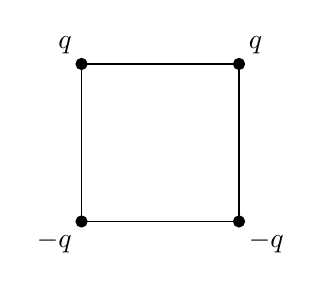
\begin{tikzpicture}
				\draw plot[mark=*,mark size = 2pt] coordinates {(0,0)(2,0)(2,2)(0,2)} -- cycle;
				\node (q) at (0,0) [below left] {$-q$};
				\node (q) at (2,0) [below right] {$-q$};
				\node (q) at (2,2) [above right] {$q$};
				\node (q) at (0,2) [above left] {$q$};
			\end{tikzpicture}
			& \hspace{.9in} &
			\begin{tikzpicture}
				\draw plot[mark=*,mark size = 2pt] coordinates {(0,0)(2,0)(2,2)(0,2)} -- cycle;
				\node (q) at (0,0) [below left] {$-q$};
				\node (q) at (2,0) [below right] {$q$};
				\node (q) at (2,2) [above right] {$-q$};
				\node (q) at (0,2) [above left] {$q$};
			\end{tikzpicture}
			\\
			(i) & & (ii)
		\end{tabular}
	\end{center}
\end{statement}

\begin{solution}
%	\hl{Jackson 9.2}
	Inspecting the figures, case~(i) is a pure dipole and case~(ii) is a pure quadrupole.  We will define the $x$ and $y$ axes such that the positive $x$ axis points toward the upper-right corner of each square, and label the charges as shown below.
	\begin{center}
		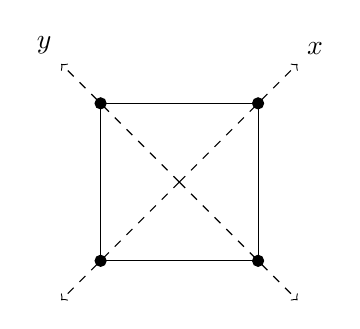
\begin{tikzpicture}
			\draw plot[mark=*,mark size = 2pt] coordinates {(0,0)(2,0)(2,2)(0,2)} -- cycle;
			\node (q) at (0,0) [above left] {$\qe$};
			\node (q) at (2,0) [above right] {$\qr$};
			\node (q) at (2,2) [below right] {$\qq$};
			\node (q) at (0,2) [below left] {$\qw$};
			\draw[dashed,->] (1,1) -- (2.5,2.5);
			\draw[dashed,->] (1,1) -- (-0.5,-0.5);
			\node (x) at (2.5, 2.5) [above right] {$x$};
			\draw[dashed,->] (1,1) -- (-0.5,2.5);
			\draw[dashed,->] (1,1) -- (2.5,-0.5);
			\node (y) at (-0.5, 2.5) [above left] {$y$};
		\end{tikzpicture}
	\end{center}
	
	We can handle case~(i) easily using the multipole expansion for the total power given by Eq.~(5.75), which goes up to dipole order:
	\beqn \label{power}
		P = \frac{2}{3 c^3} \abs{\dv[2]{\vp}{t}}^2_\ret,
	\eeqn
	where the dipole moment is defined by Eq.~(2.36),
	\beqn \label{dipole}
		\vp = \int \vx \rho \dcx.
	\eeqn
	Note that each charge is a distance $d / \sqrt{2}$ from the origin.  The locations of each of the point charges are
	\begin{align}
		\vxq(t) &= \frac{d}{\sqrt{2}} (\cos \Omg t \,\xh + \sin \Omg t \,\yh), &
		\vxw(t) &= \frac{d}{\sqrt{2}} (-\sin \Omg t \,\xh + \cos \Omg t \,\yh), \notag \\
		\vxe(t) &= \frac{d}{\sqrt{2}} (-\cos \Omg t \,\xh - \sin \Omg t \,\yh), &
		\vxr(t) &= \frac{d}{\sqrt{2}} (\sin \Omg t \,\xh - \cos \Omg t \,\yh), \label{locs}
	\end{align}
	The charge densities for the point charges are
	\begin{align*}
		\rhoq(t, \vx) &= q \, \delta(\vx - \vxq), &
		\rhow(t, \vx) &= q \, \delta(\vx - \vxw), &
		\rhoe(t, \vx) &= -q \, \delta(\vx - \vxe), &
		\rhor(t, \vx) &= -q \, \delta(\vx - \vxr).
	\end{align*}
	Then the dipole moment is
	\begin{align*}
		\vp &= \int \vx [ \rhoq(t, \vx) + \rhow(t, \vx) + \rhoe(t, \vx) + \rhor(t, \vx) ] \dcx
		= q [ \vxq(t) + \vxw(t) - \vxe(t) - \vxr(t) ] \\
		&= \sqrt{2} q d [ (\cos \Omg t - \sin \Omg t) \,\xh + (\cos \Omg t + \sin \Omg t) \,\yh ],
	\end{align*}
	and its time derivatives are
	\begin{align*}
		\dv{\vp}{t} &= \sqrt{2} q d \Omg [ -(\sin \Omg t + \cos \Omg t) \,\xh + (\cos \Omg t - \sin \Omg t) \,\yh ], \\
		\dv[2]{\vp}{t} &= \sqrt{2} q d \Omg^2 [ (\cos \Omg t - \sin \Omg t) \,\xh - (\sin \Omg t + \sin \Omg t) \,\yh ].
	\end{align*}
	Replacing $t$ with the retarded time will make no difference to the proportionalities in the above expression, since the time dependence is only in the trigonometric arguments.  Thus we have
	\beq
		P \propto \abs{\dv[2]{\vp}{t}}^2
		\propto q^2 d^2 \Omg^4,
	\eeq
	so for case~(i),
	\begin{align*}
		\nq &= \nw = 2, &
		\ne &= 4.
	\end{align*}
	
	For case~(ii), we need to go to quadrupole order in the multipole expansion.  According to the final paragraph of Sec.~5.3.1 in the course notes, the ``electric quadrupole radiation'' gives a contribution to radiated power proportional to $\abs{\dv*[3]{\Qij}{t}}^2$.  At this order, there is also a contribution to the power from ``magnetic dipole radiation'' proportional to $\abs{\dv*[2]{\vvmu}{t}}^2$, where the magnetic dipole moment $\vvmu$ is defined by (4.32),
	\beq
		\vvmu \equiv \frac{1}{2c} \int \vx \cross \vJ(\vx) \dcx.
	\eeq
	However, from (5.68),
	\beq
		\int \vJ(\vx) \dcx = \pdv{\vp}{t},
	\eeq
	and $\vp = 0$ for case~(ii).  So the ``electric quadrupole radiation'' is the only term that contributes for case~(ii), and we have
	\beq
		P \propto \abs{\dv[3]{\Qij}{t}}^2_\ret,
	\eeq
	where the quadrupole moment is defined by Eq.~(2.47),
	\beq
		\Qij = \int (3 x_i x_j - r^2 \del_{ij}) \rho \dcx.
	\eeq
	The locations of the point charges are again given by \refeq{locs}, but now their charge densities are
	\begin{align*}
		\rhoq(t, \vx) &= -q \, \delta(\vx - \vxq), &
		\rhow(t, \vx) &= q \, \delta(\vx - \vxw), &
		\rhoe(t, \vx) &= -q \, \delta(\vx - \vxe), &
		\rhor(t, \vx) &= q \, \delta(\vx - \vxr).
	\end{align*}
	Recall that $\Qij$ is symmetric.  Its elements are
	\begin{align*}
		\Qqq &= \int (3 x^2 - x^2 - y^2 - z^2) [ \rhoq(t, \vx) + \rhow(t, \vx) + \rhoe(t, \vx) + \rhor(t, \vx) ] \dcx \\
		&= q \int (2 x^2 - y^2 - z^2) [ -\delta(\vx - \vxq) + \delta(\vx - \vxw) - \delta(\vx - \vxe) + \delta(\vx - \vxr) ] \dcx \\
		&= \frac{q d^2}{2} (-2 \cos^2 \Omg t - \sin^2 \Omg t + 2 \sin^2 \Omg t + \cos^2 \Omg t - 2 \cos^2 \Omg t - \sin^2 \Omg t + 2 \sin^2 \Omg t + \cos^2 \Omg t) \\
		&= q d^2 (\sin^2 \Omg t - \cos^2 \Omg t)
		= -q d^2 \cos 2\Omg t, \\[2ex]
		Q_{12} & = 3 \int xy [ \rhoq(t, \vx) + \rhow(t, \vx) + \rhoe(t, \vx) + \rhor(t, \vx) ] \dcx \\
		&= 3q \int [ -\delta(\vx - \vxq) + \delta(\vx - \vxw) - \delta(\vx - \vxe) + \delta(\vx - \vxr) ] \dcx
		= -6 q d^2 \sin \Omg t \cos \Omg t
		= -3 q d^2 \sin 2\Omg t \\
		&= Q_{21}, \\[2ex]
		Q_{22} &= q \int (2 y^2 - x^2 - z^2) [ -\delta(\vx - \vxq) + \delta(\vx - \vxw) - \delta(\vx - \vxe) + \delta(\vx - \vxr) ] \dcx
		= q d^2 (\cos^2 \Omg t - \sin^2 \Omg t) \\
		&= -\Qqq, \\[2ex]
		Q_{13} &= Q_{23} = Q_{33} = 0.
	\end{align*}
	All of the nonzero elements have the same powers of $d$, $q$, $\cos$, and $\sin$, as we might have guessed from dimensional analysis.  Thus, we need only differentiate one of them to find the general proportionality.  Differentiating $\Qqq$ with respect to time,
	\begin{align*}
		\dv{\Qqq}{t} &= 2 q d^2 \Omg \sin 2\Omg t, &
		\dv[2]{\Qqq}{t} &= 4 q d^2 \Omg^2 \cos 2\Omg t, &
		\dv[3]{\Qqq}{t} &= -8 q d^2 \Omg^3 \sin 2\Omg t.
	\end{align*}
	Again, it makes no difference in the proportionality whether we evaluate the above at the retarded time.  Thus,
	\beq
		P \propto \abs{\dv[3]{\Qqq}{t}}^2
		\propto q^2 d^4 \Omg^6,
	\eeq
	so for case~(ii),
	\begin{align*}
		\nq &= 2, &
		\nw &= 4, &
		\ne &= 6.
	\end{align*}
	\vfix
\end{solution}